\chapter{The Fullness of God's Wrath and His Righteous Judgment (15:1--16:21)}\index{judgment}\index{wrath of God}

If the seven seals\index{seals, seven} and seven trumpets\index{trumpets, seven} have gradually unveiled the judgments\index{judgment} of God, then in Revelation 15 and 16 those judgments enter their final stage. John sees seven angels entrusted with the seven last plagues\index{plagues}. They carry seven golden bowls filled with the wrath\index{wrath of God} of God and pour them out upon the earth.

Yet before the terrible judgments unfold, John is given a vision of victory. Those who have overcome\index{overcomers} the beast\index{beast}, its image, and the number of its name stand beside a sea of glass\index{sea of glass}, holding harps given them by God. They sing the song of Moses\index{Song of Moses} and the song of the Lamb\index{Song of the Lamb}.

This sequence is profoundly significant. Before the judgments descend, John shows us the victorious people of God. Those who belong to the Lamb\index{Lamb, the} do not stand condemned beneath God's wrath; they stand secure in His keeping. They have passed through tribulation without bowing before the beast, and at last they stand before God, rejoicing in His presence and worshiping\index{worship} Him. The final vision of judgment begins, therefore, not with the triumph of evil, but with the song of a redeemed\index{redemption} people whose victory rests in God.

\section{Singing the Song of the Lamb}\index{Song of the Lamb}

\begin{ScriptureBox2}{Circle what those beside the sea of glass are holding and whose song they sing. Underline the words that describe God's deeds and ways in 15:3.}

\item[15:1] I saw in heaven another great and marvelous sign: seven angels with the seven last plagues---last, because with them God's wrath is completed.

\item[15:2] And I saw what looked like a sea of glass glowing with fire and, standing beside the sea, those who had been victorious over the beast and its image and over the number of its name. They held harps given them by God

\item[15:3] and sang the song of God's servant Moses and of the Lamb:\\
\hspace*{1em}``Great and marvelous are your deeds,\\
\hspace*{2em}Lord God Almighty.\\
\hspace*{1em}Just and true are your ways,\\
\hspace*{2em}King of the nations.
% NIV footnote for 15:3 (omitted; add as \footnote if wanted):
%   ``King of the nations'' --- Some manuscripts ages

\item[15:4] \hspace*{1em}Who will not fear you, Lord,\\
\hspace*{2em}and bring glory to your name?\\
\hspace*{1em}For you alone are holy.\\
\hspace*{1em}All nations will come\\
\hspace*{2em}and worship before you,\\
\hspace*{1em}for your righteous acts have been revealed.''
% NIV footnote for 15:4 (omitted; add as \footnote if wanted):
%   end of song --- Phrases in this song are drawn from Psalm 111:2,3;
%   Deut. 32:4; Jer. 10:7; Psalms 86:9; 98:2.
% CHECK NIV: footnote wording quoted from memory; verify against Bible Gateway.

\item[15:5] After this I looked, and I saw in heaven the temple---that is, the tabernacle of the covenant law---and it was opened.

\item[15:6] Out of the temple came the seven angels with the seven plagues. They were dressed in clean, shining linen and wore golden sashes around their chests.

\item[15:7] Then one of the four living creatures gave to the seven angels seven golden bowls filled with the wrath of God, who lives for ever and ever.

\item[15:8] And the temple was filled with smoke from the glory of God and from his power, and no one could enter the temple until the seven plagues of the seven angels were completed.

\end{ScriptureBox2}

Revelation 15 echoes Exodus 15 in striking ways. As shown in Table \ref{tab:rev_exdus_15}, when Moses\index{Moses} and the Israelites passed through the Red Sea, Pharaoh and his army were swallowed by its waters. Having witnessed God's deliverance, Moses and the people broke into a song of triumph. In Revelation 15, the song rises once more, but now it celebrates the Lamb's final victory: He has redeemed His people and overcome\index{overcomers} every power that sets itself against God.

This is not a song that celebrates human courage or achievement. It proclaims the greatness of God's works: they are “great and marvelous”; His ways are “just and true.” When suffering narrows our vision until we can see little beyond our own circumstances, this song lifts our eyes again to the Lord. The final word belongs not to the beast\index{beast}, nor to the powers that persecute\index{persecution} God's people, but to the God whose works are wonderful and whose ways are righteous.

\begin{ReaderQuestion}
In Revelation 15:3--4, the song does not celebrate human courage but proclaims that God's works are “great and marvelous” and His ways “just and true.” When suffering draws our attention toward our own circumstances, how does this song turn our eyes back to God?
\end{ReaderQuestion}

{
\small
\renewcommand{\arraystretch}{1}
\label{tab:rev_exdus_15}
\noindent
\begin{tabular}{@{}L{2.8cm} L{2.8cm} L{3.2cm}@{}}
\hline
Revelation 15 & Exodus 15 & Theme \\
\hline
Verse 1: The seven plagues & The ten plagues of Egypt & God judges His enemies \\
Verse 2: Standing beside the sea of glass & Crossing the Red Sea & God delivers His people \\
Verse 2: The beast & Pharaoh and the Egyptian army & God contends with His enemies \\
Verse 3: The song of Moses and the Lamb & The song of Moses & A song of victory after redemption \\
Verse 5: The sanctuary containing the covenant tablets & The tabernacle and sanctuary & The presence of God \\
Verse 8: Smoke filling the sanctuary & The glory of God & God's presence and judgment \\
\hline
\end{tabular}
\par
}

The angels receive their bowls and prepare to pour them out upon the earth. Below, the world is about to be struck by judgment; above, the heavenly sanctuary stands filled with the glory\index{glory} of God. No one can enter it until the seven plagues\index{plagues} entrusted to the angels have run their course. The judgment proceeding from heaven is neither accidental nor beyond God's authority. It unfolds under the sovereignty of the One whose holiness fills His sanctuary.

\section{The First Five Bowls}

\begin{figure}[htbp]
    \centering
    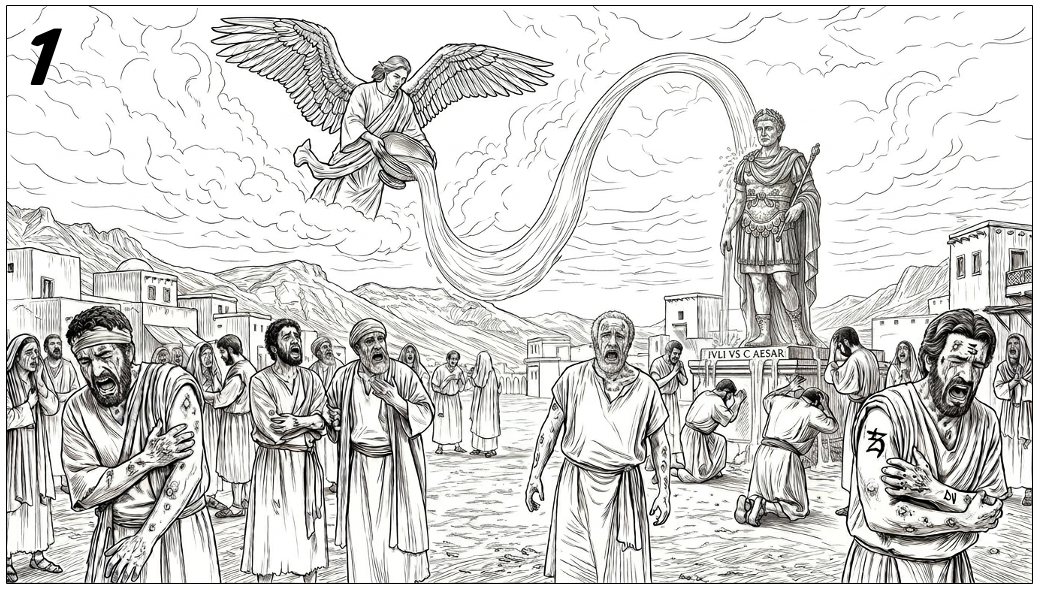
\includegraphics[
    width=1\textwidth,
    trim=0 0 0 0,
    clip]{images/bowl_1.png}
\end{figure}

\begin{figure}[htbp]
    \centering
    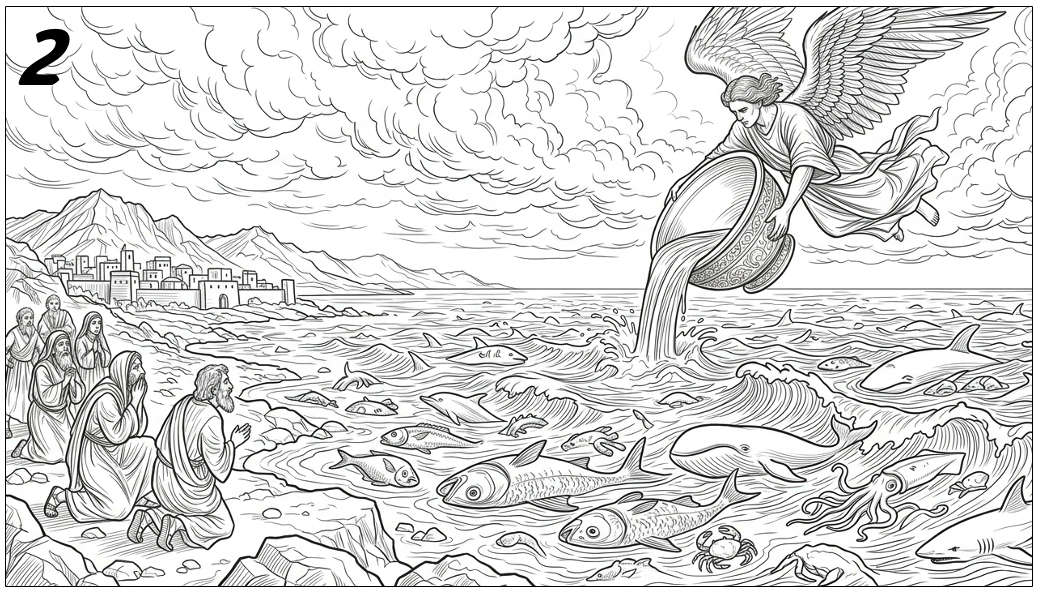
\includegraphics[
    width=1\textwidth,
    trim=0 0 0 0,
    clip]{images/bowl_2.png}
\end{figure}

\begin{ScriptureBox2}{Where is each of the first five bowls poured out? Underline how the people respond in 16:9 and 16:11.}

\item[16:1] Then I heard a loud voice from the temple saying to the seven angels, ``Go, pour out the seven bowls of God's wrath on the earth.''

\item[16:2] The first angel went and poured out his bowl on the land, and ugly, festering sores broke out on the people who had the mark of the beast and worshiped its image.

\item[16:3] The second angel poured out his bowl on the sea, and it turned into blood like that of a dead person, and every living thing in the sea died.

\item[16:4] The third angel poured out his bowl on the rivers and springs of water, and they became blood.

\item[16:5] Then I heard the angel in charge of the waters say:\\
\hspace*{1em}``You are just in these judgments, O Holy One,\\
\hspace*{2em}you who are and who were;

\item[16:6] \hspace*{1em}for they have shed the blood of your holy people and your prophets,\\
\hspace*{2em}and you have given them blood to drink as they deserve.''

\item[16:7] And I heard the altar respond:\\
\hspace*{1em}``Yes, Lord God Almighty,\\
\hspace*{2em}true and just are your judgments.''

\item[16:8] The fourth angel poured out his bowl on the sun, and the sun was allowed to scorch people with fire.

\item[16:9] They were seared by the intense heat and they cursed the name of God, who had control over these plagues, but they refused to repent and glorify him.

\item[16:10] The fifth angel poured out his bowl on the throne of the beast, and its kingdom was plunged into darkness. People gnawed their tongues in agony

\item[16:11] and cursed the God of heaven because of their pains and their sores, but they refused to repent of what they had done.

\end{ScriptureBox2}

\begin{figure}[htbp]
    \centering
    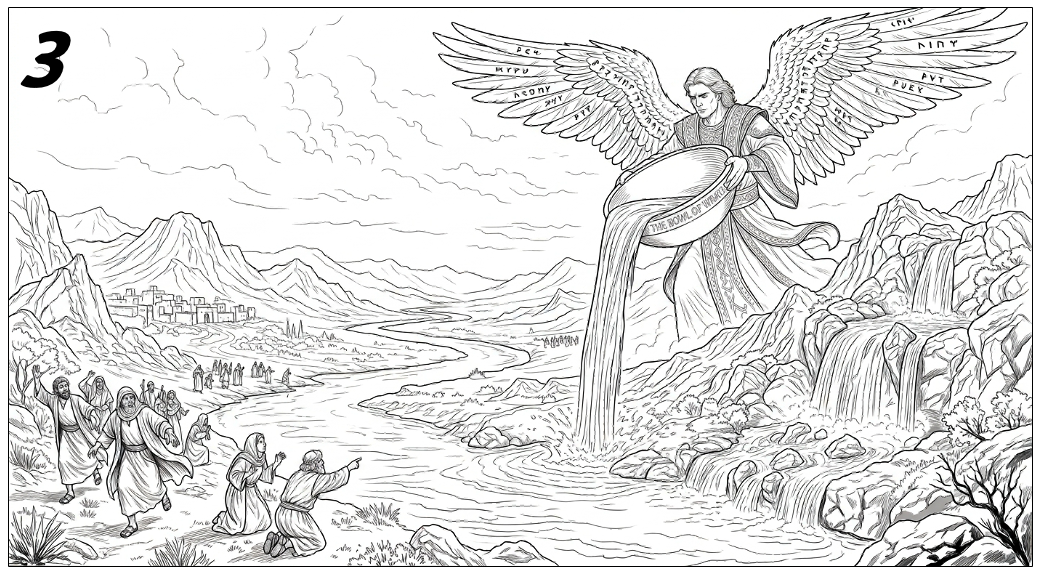
\includegraphics[
    width=1\textwidth,
    trim=0 0 0 0,
    clip]{images/bowl_3.png}
\end{figure}

The first bowl\index{bowls, seven!1@first bowl} strikes those who worship the beast\index{beast}. The second and third turn the seas and fresh waters to blood. The fourth brings scorching heat upon humanity, and the fifth plunges the beast's kingdom into darkness. The sixth bowl\index{bowls, seven!6@sixth bowl} will gather the kings of the earth for the final conflict; the seventh will announce, “It is done!” With each bowl, the judgment intensifies, until God's wrath\index{wrath of God} has been poured out in its fullness and the judgment reaches its appointed end.

These dreadful scenes do not portray the fate of those who belong to the Lamb and have been redeemed by Him. The first bowl\index{bowls, seven!1@first bowl} falls specifically upon those who bear the beast's mark and worship its image. The bowls reveal the terrible consequences of allegiance to the powers that oppose God. He has been patient for a long time, calling people repeatedly to repentance\index{repentance}. But in this vision, the appointed hour of judgment has arrived.

\begin{ReaderQuestion}
How do you understand the relationship between God's patience and His final judgment? Does God's patience mean that He takes sin lightly? Why or why not?
\end{ReaderQuestion}

\begin{figure}[htbp]
    \centering
    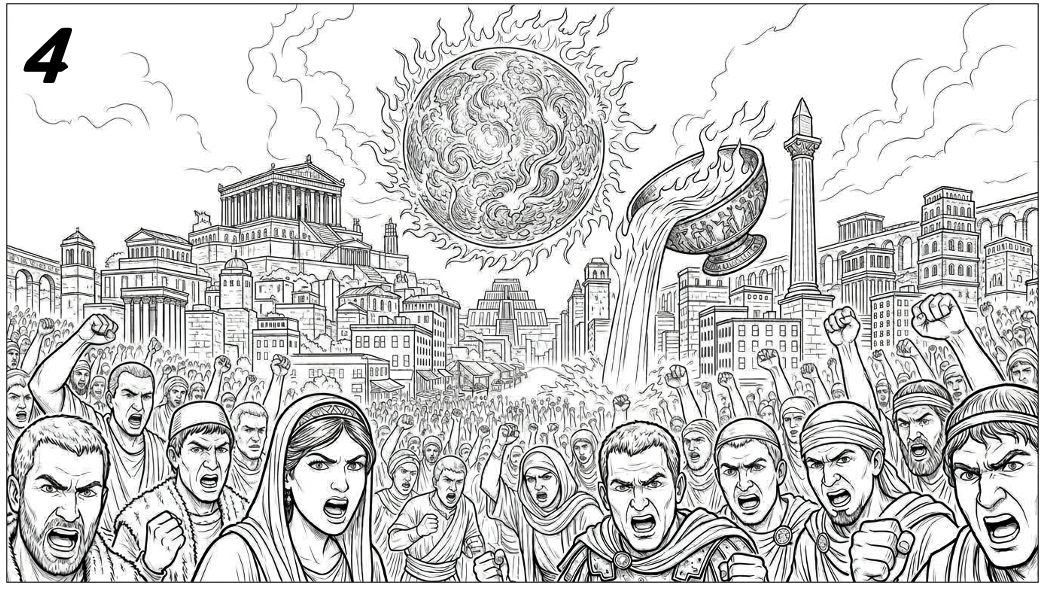
\includegraphics[
    width=1\textwidth,
    trim=0 0 0 0,
    clip]{images/bowl_4.png}
\end{figure}

At this point, we may recall the famous sermon by Jonathan Edwards, “Sinners in the Hands of an Angry God,” discussed in Chapter 10 of the first volume, \textit{Caught by Grace\index{grace}}. In forceful and unsettling language, Edwards describes the peril facing sinners who have not sought refuge in Christ:

\begin{quote}
“O sinner! Consider the fearful danger you are in: it is a great furnace of wrath, a wide and bottomless pit, full of the fire of wrath, over which you are held in the hand of that God whose wrath is provoked and incensed as much against you as against many of the damned in hell. You hang by a slender thread, with the flames of divine wrath flashing about it, ready every moment to singe it and burn it through; and you have no Mediator, no refuge to save you, no strength of your own to withstand the flames. Nothing you possess, nothing you have done, can persuade God to spare you for even a moment\ldots”
\end{quote}

Dear reader, today is still a day of grace. The Lamb has given His life for sinners. It is precisely because the coming judgment is real that the grace of God is so precious. The vision of divine wrath is not given merely to terrify us; it also summons us to seek refuge in the Savior while the invitation of grace still stands. Will you respond to God's grace and receive the salvation He offers through Christ?

\begin{ReaderQuestion}
Today is still a day of grace. How can you respond more earnestly through repentance, perseverance in faith, and trust in the Lamb? How might you share the good news of Christ with those who have not yet come to know Him?
\end{ReaderQuestion}

\begin{figure}[htbp]
    \centering
    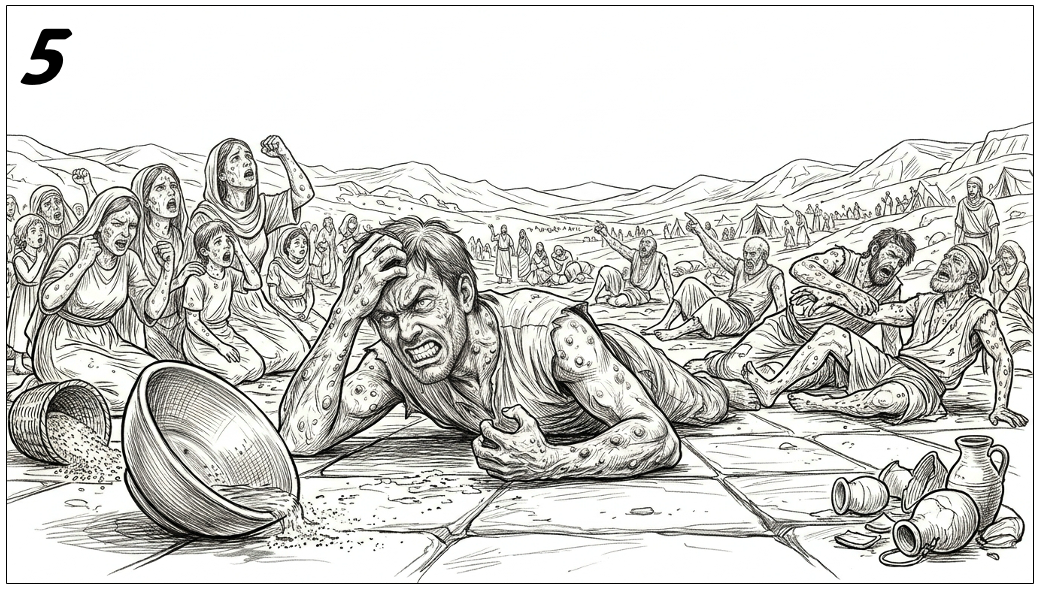
\includegraphics[
    width=1\textwidth,
    trim=0 0 0 0,
    clip]{images/bowl_5.png}
\end{figure}

\section{The Sixth Bowl}\index{bowls, seven!6@sixth bowl}

\begin{ScriptureBox2}{Out of whose mouths do the three impure spirits come, and for what do they gather the kings? What blessing does Jesus speak in 16:15?}

\item[16:12] The sixth angel poured out his bowl on the great river Euphrates, and its water was dried up to prepare the way for the kings from the East.

\item[16:13] Then I saw three impure spirits that looked like frogs; they came out of the mouth of the dragon, out of the mouth of the beast and out of the mouth of the false prophet.

\item[16:14] They are demonic spirits that perform signs, and they go out to the kings of the whole world, to gather them for the battle on the great day of God Almighty.

\item[16:15] ``Look, I come like a thief! Blessed is the one who stays awake and remains clothed, so as not to go naked and be shamefully exposed.''

\item[16:16] Then they gathered the kings together to the place that in Hebrew is called Armageddon.

\end{ScriptureBox2}

\begin{figure}[htbp]
    \centering
    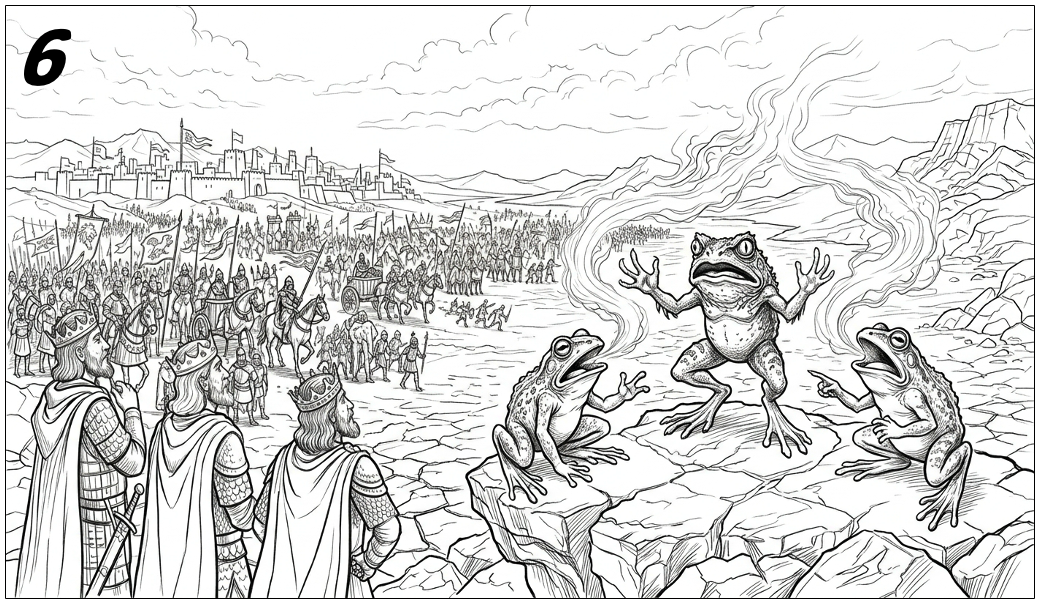
\includegraphics[
    width=1\textwidth,
    trim=0 0 0 0,
    clip]{images/bowl_6.png}
\end{figure}

Here the vision reaches one of the climactic moments of the seven bowls\index{bowls, seven}.

Three impure spirits, resembling frogs, emerge from the mouths of the dragon\index{dragon}, the beast\index{beast}, and the false prophet\index{false prophet}. They go out to deceive the kings of the earth and gather them for battle. The rulers of the nations may believe they are making their own political and military decisions. Yet John is permitted to see what lies behind the visible events: demonic spirits are deceiving them and drawing them toward the final judgment of God.

In popular novels and films about the end times\index{end times}, “Armageddon\index{Armageddon}” has become a familiar name for the great final battle. The name is generally associated with the Hebrew name Megiddo, a strategically important region in ancient Israel\index{Israel} and the site of several major conflicts. It provides a fitting symbolic setting for John's vision of the final confrontation between the powers opposed to God and the Lord who reigns over all.

Revelation 16:16 describes the gathering of the hostile earthly powers at the place called Armageddon\index{Armageddon}. The battle itself is portrayed more fully in Revelation 19:19--21. This is no contest between two evenly matched forces. Christ's victory is decisive. The forces of evil may gather in defiance of God, but they cannot overturn His sovereignty or escape His judgment.

Because the vision spans these two chapters, Figure \ref{rev_16_19_armageddon_english} presents the connection between them. It also illustrates how Satan\index{Satan} works through the three frog-like spirits to incite those who follow him on earth to oppose God. Yet Satan knows that his time is short. As Revelation 12:12 declares, his fury is great because he knows that his time is limited. His rage does not signal strength sufficient to prevail; it reveals the desperation of a defeated enemy whose end is approaching.

\begin{figure}[htbp]
    \centering
    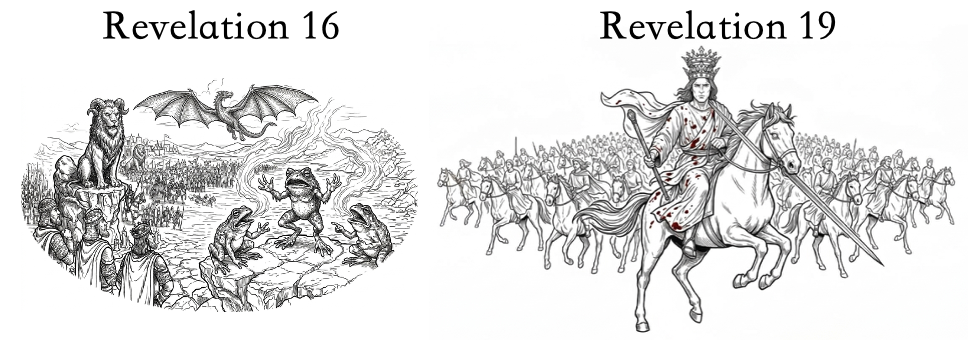
\includegraphics[
    width=1\textwidth,
    trim=0 10 20 0,
    clip]{images/rev_16_19_armageddon_english.png}
    \caption{The Battle of Armageddon}
    \label{rev_16_19_armageddon_english}
\end{figure}

\section{The Seventh Bowl}\index{bowls, seven!7@seventh bowl}

\begin{ScriptureBox2}{What does the loud voice from the throne declare? Circle every sign that follows, and notice how the people respond to the hail.}

\item[16:17] The seventh angel poured out his bowl into the air, and out of the temple came a loud voice from the throne, saying, ``It is done!''

\item[16:18] Then there came flashes of lightning, rumblings, peals of thunder and a severe earthquake. No earthquake like it has ever occurred since mankind has been on earth, so tremendous was the quake.

\item[16:19] The great city split into three parts, and the cities of the nations collapsed. God remembered Babylon the Great and gave her the cup filled with the wine of the fury of his wrath.

\item[16:20] Every island fled away and the mountains could not be found.

\item[16:21] From the sky huge hailstones, each weighing about a hundred pounds, fell on people. And they cursed God on account of the plague of hail, because the plague was so terrible.
% NIV footnote for 16:21 (omitted; add as \footnote if wanted):
%   ``a hundred pounds'' --- Or about 45 kilograms
% CHECK NIV: footnote wording quoted from memory; verify against Bible Gateway.

\end{ScriptureBox2}

The most important words in this final scene are the declaration from the throne\index{throne of God}: “It is done!” God's judgment has reached its appointed completion. Yet even as the earth is shaken to its foundations, humanity's rebellion remains stubbornly unchanged.

The earthquake\index{earthquake} is unlike any that has occurred since humanity first appeared on the earth. Hailstones weighing about a talent—approximately 45 kilograms, or 100 pounds—fall from the sky. The devastation is immense, yet the people still blaspheme God. Even in the face of overwhelming judgment, they refuse to turn to Him in repentance\index{repentance}.

This brings to mind a passage from \textit{The Great Divorce} by C. S. Lewis, quoted in Chapter 12 of the first volume, \textit{Caught by Grace}:

\begin{quote}
“There are only two kinds of people in the end: those who say to God, ‘Thy will be done,’ and those to whom God says, in the end, ‘Thy will be done.’ All that are in Hell, choose it. Without that self-choice there could be no Hell. No soul that seriously and constantly desires joy will ever miss it. Those who seek find. Those who knock it is opened.”
\footnote{Lewis, C. S. (1946). \textit{The Great Divorce}. Geoffrey Bles.}
\end{quote}

The final bowls reveal more than the destruction of the world as we know it. They expose the gravity of humanity's persistent refusal to yield to God. The question is not simply whether people will witness God's power, but whether they will humble themselves before Him. 

\begin{ReaderQuestion}
C. S. Lewis wrote that in the end there are only two kinds of people: those who say to God, ``Thy will be done,'' and those to whom God says, ``Thy will be done.'' In what area of your life are you still holding on to your own will? What would it look like to say to God today, ``Thy will be done''?
\end{ReaderQuestion}

\section*{The Seven Bowls at a Glance}\index{bowls, seven}

The following mnemonic summarizes the distinctive features of the seven bowls\index{bowls, seven} and makes them easier to remember.

{
\small
\renewcommand{\arraystretch}{1}
\begin{longtable}{>{\raggedright\arraybackslash}p{1.5cm}
                  >{\raggedright\arraybackslash}p{2cm}
                  >{\raggedright\arraybackslash}p{4cm}}
\caption{The seven bowls}
\label{tab:seven-bowls} \\
\hline
Bowl & Passage & Judgment \\
\hline
\endfirsthead

\multicolumn{3}{l}{\small\itshape Table~\thetable\ (continued)} \\
\hline
Bowl & Passage & Judgment \\
\hline
\endhead

\hline
\endfoot

\hline
\endlastfoot

First   & 16:1--2   & Sores spread \\
Second  & 16:3      & Sea red \\
Third   & 16:4--7   & Rivers bled \\
Fourth  & 16:8--9   & Sun's heat \\
Fifth   & 16:10--11 & Beast's dark seat \\
Sixth   & 16:12--16 & War begun \\
Seventh & 16:17--21 & ``It is done!'' \\
\end{longtable}
}
